\section{Tool functions}


\subsection{xlpArgs}

\begin{xlpfunctitle}{xlpArgs}

\begin{xlpfunc}{Parameters}
\begin{tabular}{p{3.5cm}cl}
\textbf{args01}& : & cell list arguments 01 \\
\textbf{args02}& : & cell list arguments 02 \\
\textbf{args03}& : & cell list arguments 03 \\
\textbf{args04}& : & cell list arguments 04 \\
\textbf{args05}& : & cell list arguments 05 \\
\textbf{transpose}& : & transpose \\
\textbf{trigger}& : & trigger 
\end{tabular}
\end{xlpfunc}


\begin{xlpfunc}{Returns}
A cell matrix of dimension (n, 1) where n is the sum of the size of all list arguments.
\end{xlpfunc}

\begin{xlpfunc}{Description}
This function allows to concatenate various cell lists into one cell list.
This function is dedicated to be used in the call to other functions as {\it args} parameter.

Imagine that you have a volatiliy term structure depending on time and strike. Imagine that your object has an associated method called {\it blackVol} taking two parameters, time and strike. You want to fill a grid of volatilities like in the image below:

\

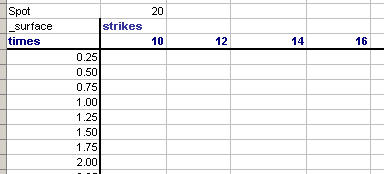
\includegraphics[width=11cm]{images/surface.jpg}

The function call in each cell will be similar to:

\begin{center}
{\sl xlpGetAttr($A$38,"blackVol",xlpArgs($A40,B$39, $B$37),,$C$21)}
\end{center}

\

Where you can see the usage of xlpArgs to create a cross reference args parameter from the times and the strikes. 

\

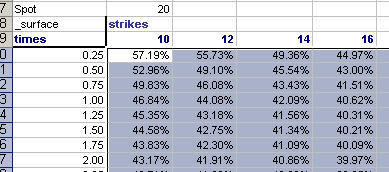
\includegraphics[width=11cm]{images/surface3.jpg}
\end{xlpfunc}
\end{xlpfunctitle}


\subsection{xlpBigArgs}

\begin{xlpfunctitle}{xlpBigArgs}

\begin{xlpfunc}{Parameters}
\begin{tabular}{p{3.5cm}cl}
\textbf{args01}& : & cell list arguments 01 \\
\textbf{args02}& : & cell list arguments 02 \\
\textbf{args03}& : & cell list arguments 03 \\
\textbf{args04}& : & cell list arguments 04 \\
\textbf{args05}& : & cell list arguments 05 \\
\textbf{args06}& : & cell list arguments 06 \\
\textbf{args07}& : & cell list arguments 07 \\
\textbf{args08}& : & cell list arguments 08 \\
\textbf{args09}& : & cell list arguments 09 \\
\textbf{args10}& : & cell list arguments 10 \\
\textbf{args11}& : & cell list arguments 11 \\
\textbf{args12}& : & cell list arguments 12 \\
\textbf{args13}& : & cell list arguments 13 \\
\textbf{args14}& : & cell list arguments 14 \\
\textbf{args15}& : & cell list arguments 15 \\
\textbf{args16}& : & cell list arguments 16 \\
\textbf{args17}& : & cell list arguments 17 \\
\textbf{args18}& : & cell list arguments 18 \\
\textbf{transpose}& : & transpose \\
\textbf{trigger}& : & trigger 
\end{tabular}
\end{xlpfunc}


\begin{xlpfunc}{Returns}
A cell matrix of dimension (n, 1) where n is the sum of the size of all list arguments.
\end{xlpfunc}

\begin{xlpfunc}{Description}
Like xlpArgs.
\end{xlpfunc}
\end{xlpfunctitle}


\subsection{xlpTranspose}

\begin{xlpfunctitle}{xlpTranspose}

\begin{xlpfunc}{Parameters}
\begin{tabular}{p{3.5cm}cl}
\textbf{scalars}& : & cell matrix \\
\textbf{trigger}& : & trigger 
\end{tabular}
\end{xlpfunc}


\begin{xlpfunc}{Returns}
A cell matrix of dimension (m, n) where n is the number of rows and m the number of columns of the imput cell matrix.
\end{xlpfunc}

\begin{xlpfunc}{Description}
Transpose a cell matrix.
\end{xlpfunc}
\end{xlpfunctitle}




\subsection{xlpTrigger}

\begin{xlpfunctitle}{xlpTrigger}

\begin{xlpfunc}{Parameters}
\begin{tabular}{p{3.5cm}cl}
\textbf{trigger01}& : & trigger 01 \\
\textbf{trigger02}& : & trigger 02 \\
\textbf{trigger03}& : & trigger 03 \\
\textbf{trigger04}& : & trigger 04 \\
\textbf{trigger05}& : & trigger 05 \\
\end{tabular}
\end{xlpfunc}


\begin{xlpfunc}{Returns}
An index.
\end{xlpfunc}

\begin{xlpfunc}{Description}
Return FALSE if one of the trigger is in error or FALSE. Otherwise it return an incressing index.
\end{xlpfunc}
\end{xlpfunctitle}

\subsection{xlpBigTrigger}

\begin{xlpfunctitle}{xlpBigTrigger}

\begin{xlpfunc}{Parameters}
\begin{tabular}{p{3.5cm}cl}
\textbf{trigger01}& : & trigger 01 \\
\textbf{trigger02}& : & trigger 02 \\
\textbf{trigger03}& : & trigger 03 \\
\textbf{trigger04}& : & trigger 04 \\
\textbf{trigger05}& : & trigger 05 \\
\textbf{trigger06}& : & trigger 06 \\
\textbf{trigger07}& : & trigger 07 \\
\textbf{trigger08}& : & trigger 08 \\
\textbf{trigger09}& : & trigger 09 \\
\textbf{trigger10}& : & trigger 10 \\
\textbf{trigger11}& : & trigger 11 \\
\textbf{trigger12}& : & trigger 12 \\
\textbf{trigger13}& : & trigger 13 \\
\textbf{trigger14}& : & trigger 14 \\
\textbf{trigger15}& : & trigger 15 \\
\textbf{trigger16}& : & trigger 16 \\
\textbf{trigger17}& : & trigger 17 \\
\textbf{trigger18}& : & trigger 18 \\
\textbf{trigger19}& : & trigger 19 \\
\textbf{trigger20}& : & trigger 20 \\
\end{tabular}
\end{xlpfunc}


\begin{xlpfunc}{Returns}
An index.
\end{xlpfunc}

\begin{xlpfunc}{Description}
Return FALSE if one of the trigger is in error or FALSE. Otherwise it return an incressing index.
\end{xlpfunc}
\end{xlpfunctitle}


\subsection{xlpTranspose}

\begin{xlpfunctitle}{xlpTranspose}

\begin{xlpfunc}{Parameters}
\begin{tabular}{p{3.5cm}cl}
\textbf{scalars}& : & cell matrix \\
\textbf{trigger}& : & trigger 
\end{tabular}
\end{xlpfunc}


\begin{xlpfunc}{Returns}
A cell matrix of dimension (m, n) where n is the number of rows and m the number of columns of the imput cell matrix.
\end{xlpfunc}

\begin{xlpfunc}{Description}
Transpose a cell matrix.
\end{xlpfunc}
\end{xlpfunctitle}




\subsection{xlpAdjustShape}

\begin{xlpfunctitle}{xlpAdjustShape}

\begin{xlpfunc}{Parameters}
\begin{tabular}{p{3.5cm}cl}
\textbf{scalars}& : & cell matrix \\
\textbf{rows}& : & number of rows \\
\textbf{columns}& : & number of columns \\
\textbf{trigger}& : & trigger 
\end{tabular}
\end{xlpfunc}


\begin{xlpfunc}{Returns}
A cell matrix of dimension (rows, columns) where $rows * columnns$ is  equal to $rows\_input\_matrix * columns\_input\_matrix$.  
\end{xlpfunc}

\begin{xlpfunc}{Description}
Transpose a cell matrix.
\end{xlpfunc}
\end{xlpfunctitle}


\subsection{xlpLoadFile}

\begin{xlpfunctitle}{xlpLoadFile}

\begin{xlpfunc}{Parameters}
\begin{tabular}{p{3.5cm}cl}
\textbf{file}& : & filename \\
\textbf{id}& : & object id \\
\textbf{trigger}& : & trigger 
\end{tabular}
\end{xlpfunc}


\begin{xlpfunc}{Returns}
A character string representing the object id
\end{xlpfunc}

\begin{xlpfunc}{Description}
Load a file referenced by filename and store it as a character string python object. 
\end{xlpfunc}
\end{xlpfunctitle}


\subsection{xlpVolatile}

\begin{xlpfunctitle}{xlpVolatile}

\begin{xlpfunc}{Parameters}
\begin{tabular}{p{3.5cm}cl}
\textbf{trigger}& : & trigger 
\end{tabular}
\end{xlpfunc}


\begin{xlpfunc}{Returns}
A real number.
\end{xlpfunc}

\begin{xlpfunc}{Description}
The function return a incremental number. This function is volatile, that mean that Excel calls it every time that a change occureds on the sheet.
\end{xlpfunc}
\end{xlpfunctitle}

\subsection{xlpReduce}

\begin{xlpfunctitle}{xlpReduce}

\begin{xlpfunc}{Parameters}
\begin{tabular}{p{3.5cm}cl}
\textbf{args}& : & arguments \\
\textbf{transpose}& : & output transpose \\
\textbf{trigger}& : & trigger 
\end{tabular}
\end{xlpfunc}


\begin{xlpfunc}{Returns}
A cell matrix.
\end{xlpfunc}

\begin{xlpfunc}{Description}
The function reduce a cell matrix into another matrix eliminating the error or missing cell. This function can handle only matrix where there is full rows or full columns in error.
\end{xlpfunc}
\end{xlpfunctitle}


\subsection{xlpR}

\begin{xlpfunctitle}{xlpR}

\begin{xlpfunc}{Parameters}
\begin{tabular}{p{3.5cm}cl}
\textbf{args}& : & arguments \\
\textbf{transpose}& : & output transpose \\
\textbf{trigger}& : & trigger 
\end{tabular}
\end{xlpfunc}


\begin{xlpfunc}{Returns}
A cell matrix.
\end{xlpfunc}

\begin{xlpfunc}{Description}
Shortcut for xlpReduce.
\end{xlpfunc}
\end{xlpfunctitle}


\subsection{xlpPretty}

\begin{xlpfunctitle}{xlpPretty}

\begin{xlpfunc}{Parameters}
\begin{tabular}{p{3.5cm}cl}
\textbf{args}& : & arguments \\
\textbf{transpose}& : & output transpose \\
\textbf{trigger}& : & trigger 
\end{tabular}
\end{xlpfunc}


\begin{xlpfunc}{Returns}
A cell matrix.
\end{xlpfunc}

\begin{xlpfunc}{Description}
Get a pretty matrix. This function cannot be called inside another \xlp function.
Try it for explanation.
\end{xlpfunc}
\end{xlpfunctitle}


\subsection{xlpP}

\begin{xlpfunctitle}{xlpP}

\begin{xlpfunc}{Parameters}
\begin{tabular}{p{3.5cm}cl}
\textbf{args}& : & arguments \\
\textbf{transpose}& : & output transpose \\
\textbf{trigger}& : & trigger 
\end{tabular}
\end{xlpfunc}


\begin{xlpfunc}{Returns}
A cell matrix.
\end{xlpfunc}

\begin{xlpfunc}{Description}
Shortcut for xlpPretty.
\end{xlpfunc}
\end{xlpfunctitle}

\subsection{xlpTime}

\begin{xlpfunctitle}{xlpTime}

\begin{xlpfunc}{Parameters}
\begin{tabular}{p{3.5cm}cl}
\textbf{trigger}& : & trigger 
\end{tabular}
\end{xlpfunc}


\begin{xlpfunc}{Returns}
A real number.
\end{xlpfunc}

\begin{xlpfunc}{Description}
Return a real number representing the time in second since the add-in has been loaded. 
The aim of this function is to allow calculating execution time of a function.
\end{xlpfunc}
\end{xlpfunctitle}

